\chapterimage{head2.png} % Chapter heading image
\chapter{Convex Sets}
\section{Convexity}
\subsection{Cone}
\begin{definition}[Cone]
A set $K \in \R^n$, when $x \in K $ implies $\alpha x \in K$.
\end{definition}
A non convex cone can be hyper-plane.\\
For convex cone $x + y \in K, \forall x,y \in K$.\\
Cone don't need to be "pointed". e.g. \\
Direct sums of cones $C_1 + C_2 = \{ x = x_1+x_2 | x_1 \in C_1, x_2 \in C_2 \}$.\\
\begin{example}
$S_1^n  \{ X | X=X^n ,\lambda(x) \ge 0\}$\\
A matrix with positive eigenvalues.
\end{example}

\subsubsection{Operations preserving convexity}
\begin{itemize}
\item[Intersection] $C  \cap_{i \in \mathbb{I}}C_i$
\item[Linear map] Let $A : \mathbb{R}^n \to  \R^n$ be a linear map. If $C \in \R^n$ is convex, so is $A(C) = \{Ax \forall x \in C \}$
\item[Inverse image] $A^{-1}(D) = \{ x \in \R |Ax \in D \}$
\end{itemize}

\subsubsection{Operations that induce convexity}
Convex hull on $S = \cap \{C | S\in C, C is convex\}$\\
\begin{example}
$Co \{ x_1,x_2,\cdots,x_m\} = \{ \sum_{i=1}^m \alpha_i x_i | \alpha \in \delta_m \}$
\end{example}
For a convex set $x \in C \Rightarrow x = \sum \alpha_i x_i$. 
\begin{theorem}[Carathéodory's theorem]
If a point $x \in \R^d$ lies in the convex hull of a set $P$, there is a subset $P'$ of $P$ consisting of $d + 1$ or fewer points such that $x$ lies in the convex hull of $P'$. Equivalently, x lies in an r-simplex with vertices in P.
\end{theorem}

\section{Convex Functions}
\begin{definition}[Convex function]
Let $C \in \R^n$ be convex, $f:C \to \R$ is convex on f if $x,y \in C \times C$. $\forall \alpha \in (0,1)$, $f(\alpha x + (1-\alpha) y) \le f(\alpha x) + f((1-\alpha) y)$
\end{definition}

\begin{definition}[Strictly Convex function]
Let $C \in \R^n$ be convex, $f:C \to \R$ is strictly convex on f if $x,y \in C \times C$. $\forall \alpha \in (0,1)$, $f(\alpha x + (1-\alpha) y) \langle f(\alpha x) + f((1-\alpha) y)$
\end{definition}

\begin{definition}[Strongly convex]
$f:C \to \R$ is strongly convex with modules $u \ge 0$ if $f - \frac{1}{2}u || \cdot ||^2$ is convex.
\end{definition}
Interpretation: There is a convex quadratic $\frac{1}{2}u || \cdot ||^2$ that lower bounds f.
\begin{example}
$\min_{x \in C} f(x) \leftrightarrow \min \bar{f}(x)$
Useful to turn this into an unconstrained problem. \\
$$\bar{f}(x) = \begin{cases}
f(x) \quad if x \in C \\
\infty \quad  elsewhere
\end{cases}$$
\end{example}
\begin{definition}
A function $f : \R^n \to \R \cup \infty \ \bar{\R}$ is convex if $x,y \in \R^n \times \R^n$, $\forall x,y , \bar{f}(\alpha x + (1-\alpha) y) \le f(\alpha x) + f((1-\alpha) y)$
\end{definition}
Definition 1 is equivalent to definition 2 if $f(x) = \infty$.
\begin{example}
$f(x) = \sup_{j \in J} f_j(x)$
\end{example}

\subsection{Epigraph} 
\begin{definition}[Epigraph]
For $f: \R^n \rightarrow \bar{R}$, its epigraph $epi(f) \in \R^{n+1} is the set epi(f) \{ (x,\alpha) | f(x) \in \alpha \}$
\end{definition}
Next: a function is convex i.f.f. its epigraph is convex.

\begin{definition}
A function $f : C \rightarrow \R, C \in \R^n$ is convex if $\forall x, y \in C$, $f(ax + (1-a)x) \le af(x) + (1-a)f(x) \quad \forall a \in (0,1)$.\\ 
Strict convex: $x \neq y \Rightarrow f(ax + (1-a)x) \le af(x) + (1-a)f(x) $
\end{definition}
\begin{remark}
$f$ is convex $\Rightarrow$ $-f$ is concave.
\end{remark}
Level set: $S_{\alpha}f = \{ x | f(x) \le \alpha \}$.\\ 
$S_{\alpha}f$ is convex $\Leftrightarrow$ $f$ is convex. \\
\begin{definition}[Strongly convex]
$f : C \rightarrow \R$ is strongly convex with modules $\mu$ if $\forall x, y \in C$, $\forall \alpha \in (0,1)$, $f(ax + (1-a)x) \le af(x) + (1-a)f(x) - \frac{1}{2\mu}\alpha(1- \alpha) \|x-y\|^2$.
\end{definition}

\begin{remark}
\begin{itemize}
\item $f$ is 2nd-differentiable, $f$ ix \cvx $\iff$ $\nabla^2f(x) \rangle  0$.
\item $f$ is strongly \cvx $\iff$ $\nabla^2f(x) \rangle  \mu I$ $\iff$ $x \ge \mu$
\end{itemize}
\end{remark}
\begin{definition}[2]
$f : \R^n \to \bar{\R} $ is \cvx  if $x, y  \in \R , \alpha \in (0,1), f(ax + (1-a)x) \le af(x) + (1-a)f(x)$.  
\end{definition}
The effective domain of $f$ is $dom f = \{x | f(x) \langle + \infty \}$ 
\begin{example}[ludcator function]
$\delta_c(x) = \begin{cases}
0 \quad  x \in C \\
+ \infty \quad elsewhere
\end{cases}$.\\
$dom \space \delta_c(x) = C$
\end{example}
\begin{definition}[Epigraph]
The epigraph of f is $epi \space f = \{(x,\alpha) | f(x) \le \alpha\}$
\end{definition}
The graph of $epi \space f$ is $\{ (x,f(x) | x \in dom \space f\}$.
\begin{definition}[III]
A function $f : \R^n \to \bar{\R}$ is %\cvx  if $\epi \space f $ is \cvx
\end{definition}
\begin{theorem}
$f : \R^n \to \bar{\R}$ is \cvx  $\iff$ $\forall x,y \in \R^n, \alpha \in (0,1), f(ax + (1-a)x) \le af(x) + (1-a)f(x)$.
\end{theorem}
\begin{proof}
$\Rightarrow$ take $x,y \in dom \space f$, $(x,f(x)) \in epi \space f$,$(y,f(y)) \in epi \space f$.
\end{proof}

\begin{example}[Distance]
Distance to a \cvx  set $d_c(x) = \inf \{ \| z-x \| | z \in C \}$. Take any two sequence $\{ y_k\} and \{ \bar{y}_k\} \subset C$ s.t. $\| y_k - x\| \to d_c(x)$, $\| \bar{y}_k - \bar{x}\| \to d_c(\bar{x})$. $z_k = \alpha y_k + (1 - \alpha) \bar{y}_k$.
\begin{align*}
d_c(\alpha x + (1-\alpha) \bar{x}) &\le \| z_k - \alpha x - (1 - \alpha) \bar{x}\| \\
& = \| \alpha(y_k - x) + (1 - \alpha)(\bar{y}_k - \bar{x})\| \\
& \le \alpha \| y_k - x\| + (1 - \alpha ) \|\bar{y}_k - \bar{x}\|
\end{align*}
Take $k \to \infty$, $d_c(\alpha x + (1 - \alpha) \bar{x}) \le \alpha d(x) + (1 - \alpha) d(\bar{x})$
\end{example}
\begin{example}[Eigenvalues]
Let $X \in S^n := \{ n \times n symmetric matrix\}$. $\lambda_1(x) \ge \lambda_2(X) \ge \ldots \ge \lambda_n(x)$.\\
$f_k(x) = \sum_{1}^n \lambda_i(x)$.\\
Equivalent characterization 

\begin{align*}
f_k(x) & = \max\{ \sum_{i} v_i^T Xv_i | v_i \perp v_j , i \neq j\} \\
& =  \max\{ tr( V^TXV | V^T V = I_k \} \\
\max \{tr(VV^TX) \} \text{by circularity}
\end{align*}
Note $\langle A,B\rangle  = tr(A,B)$ is true for symmetric matrix. \\
$\langle A,A\rangle  = |A |_F^2 = \sum_{i} A_{ii}^2$
\end{example}

\section{Support Function}
Take a set $C \in \R^n$, not necessarily convex.The support function is $\sigma_C = \R^n \to \bar{\R}$. $\sigma_C(x) = \sum \{ \langle x,u\rangle  | u \in C\}$.
\includegraphics[scale=0.5]{1_1.png}
\begin{fact}
The support function binds the supporting hyper-plane.
\end{fact}

Supporting functions are
\begin{itemize}
\item Positively homogeneous\\
$\sigma_C(\alpha x) = \alpha \sigma_C(x) \forall \alpha \rangle  0$ \\
$\sigma_C(\alpha x ) = \sup_{u \in C} \langle \alpha x, u\rangle  = \alpha \sup_{u \in C} \langle x, u\rangle  = \alpha \sigma_C(x)$
\item Sub-linear( a special case of convex, linear combination holds $\forall \alpha$.\\
$\sigma_C(\alpha x + (1 - \alpha) y ) = \sup_{u \in C} \langle \alpha x + (1 - \alpha) y,u\rangle  \le \alpha\sup_{u \in C}\langle x,u\rangle  + (1 - \alpha)\sup_{u \in C}\langle y,u\rangle  $
\end{itemize}
\begin{example}[L2-norm]
$\| x \| = \sup_{u \in C} \{ \langle x, u \rangle, u \in \R^n \}$.\\
$\|x \|_p = \sup \{ \langle x, u \rangle, u \in B_q \}$ where $\frac{1}{p} + \frac{1}{q} = 1$. $B_q = \{ \|x \|_q \le 1\}$.\\
The norm is 
\begin{itemize}
\item Positive homogeneous
\item sub-linear
\item If $0 \in C$, $\sigma_C$ is non-negative.
\item If $C$ is central-symmetric, $\sigma_C(0) = 0$ and $\sigma_C(x) = \sigma_C(-x)$
\end{itemize}
\end{example}

\begin{fact}[Epigraph of a support function]
$epi \space \sigma_C = \{ (x,t) | \sigma_C(x) \le t\}$.
Suppose $(x,t) \in epi \space \sigma_C$. Take any  $\alpha > 0$. $\alpha(x,t) = (\alpha x, \alpha t)$.\\
$\alpha \sigma_C(x) = \alpha \sigma_C(x) \le \alpha t$. $\alpha(x,c) \in epi 
\sigma_C$\\
\includegraphics[]{1_2}
\end{fact}

\section{Operations Preserve Convexity of Functions}
\begin{itemize}
\item Positive affine transformation \\
$f_1,f_2,\ldots,f_k \in \space cvx \R^n$.\\
$f = \alpha_1 f_1 + \alpha_2 f_2 + \ldots + \alpha_k f_k$
\item Supremum of functions. Let $\{ f_i \}_{i \in I}$ be arbitrary family of functions. If $\exists x \sup_{j \in J} f_j(x) < \infty \Leftrightarrow f(x) = \sup_{j \in J} f_j(x) $\\
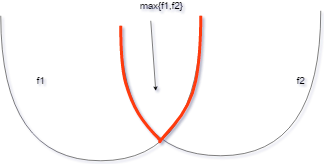
\includegraphics[]{1_3}
\item Composition with linear map.\\
$f \in cvx \R^n$, $A:\R^n \to \R^m$ is a linear map.
$f \circ A (x) = f(Ax) \in cvx \R^n$\\
\begin{align*}
f \circ A (x) & = f(A(\alpha x + (1-\alpha) y)) \\
& = f(A \alpha x + (1-\alpha) A y) \\
& \le \alpha f(Ax) + (a - \alpha) f(Ay)
\end{align*}
\end{itemize}